\documentclass[accentcolor=tud1d,colorbacktitle,inverttitle,landscape,german,presentation,t]{tudbeamer}
\usepackage[latin1]{inputenc}
\usepackage[english]{babel}
\usepackage{amsmath}
\usepackage{amsfonts}
\usepackage{amssymb}
\usepackage{graphicx}
\usepackage{multicol}

\begin{document}
	
	\title[DDPG]{Deep Deterministic Policy Gradients -\\ Components and Extensions}
	\subtitle{Yannik Frisch\\Tabea Wilke\\Maximilian Gehrke \\\\Group 19 Oleg Arenz}
	
	\author[Yannik Frisch et al.]{Yannik Frisch, Tabea Wilke and Maximilian Gehrke}
	\institute[IAS TU Darmstadt | Group 19]{Institute for Intelligent 
	Autonomous 
	Systems, TU Darmstadt}


	\logo{
\includegraphics{iasLogo}}
	% \logo{\color{tudtextaccent}\large IFP}
	
	\date{March 22, 2019}
	

\begin{titleframe}
\end{titleframe}
\section{Deep Deterministic Policy Gradient}
	\begin{frame}
		\frametitle{\\Deep Deterministic Policy Gradient}
		\begin{itemize}
			\item \textbf{Actor-Critic Method}
			\begin{itemize}
				\item Approximated critic $Q(s,a|\theta^Q)$
				\item Approximated actor $\pi(s|\theta^\pi)$
			\end{itemize}
			\vspace{2mm}
			\item \textbf{Deep Q-Learning}
			\begin{itemize}
				\item Q-Learning with approximated critic by nn
				\item $\nabla_{\theta^Q}J(\theta^Q)\approx{\rm I\!E} \left[\left(r+\gamma \max_{a'} Q(s', 
				a'|\theta^Q)-Q(s,a|\theta^Q)\right)\nabla_{\theta^Q}Q(s,a|\theta^Q)\right] $
				\item Experience Replay Buffer
				\item Target Network(s)
			\end{itemize}
			\vspace{2mm}
			\item \textbf{Deterministic Policy Gradient}
			\begin{itemize}
				\item $\nabla_{\theta^\pi}J(\theta^\pi)\approx {\rm I\!E}\left[\nabla_aQ(s,a)|_{a=\pi(s|\theta^\pi)} \nabla_{\theta^\pi}\pi(s|\theta^\pi)\right]$
				\item Enables to learn a deterministic policy while following a \\stochastic exploratory policy
			\end{itemize}
		\end{itemize}
	\end{frame}
	\begin{frame}
		\frametitle{\\DDPG Pseudocode}
		\centering
		%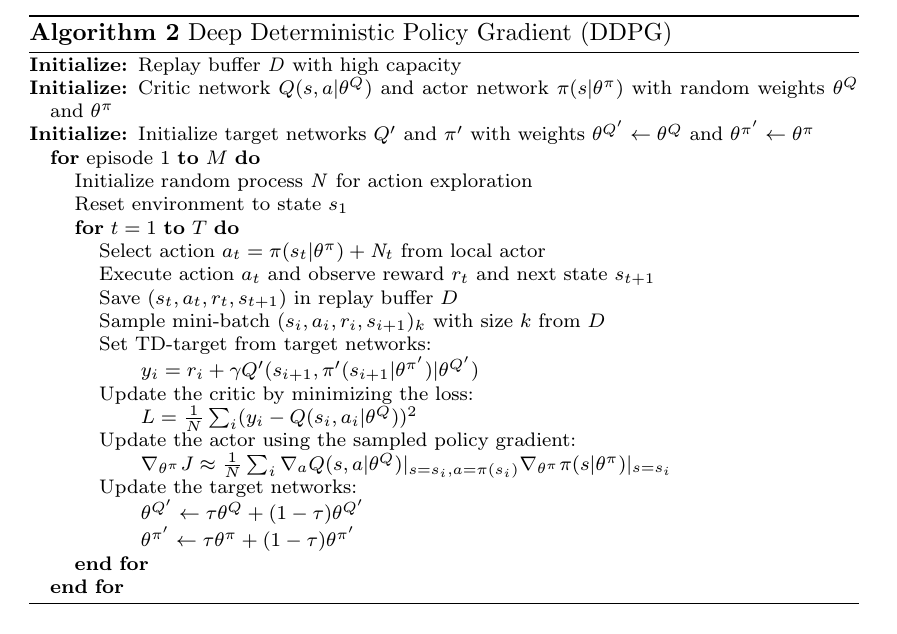
\includegraphics[scale=0.28]{ddpg_pseudocode_alt.png}
		\vspace{-4.5mm}
		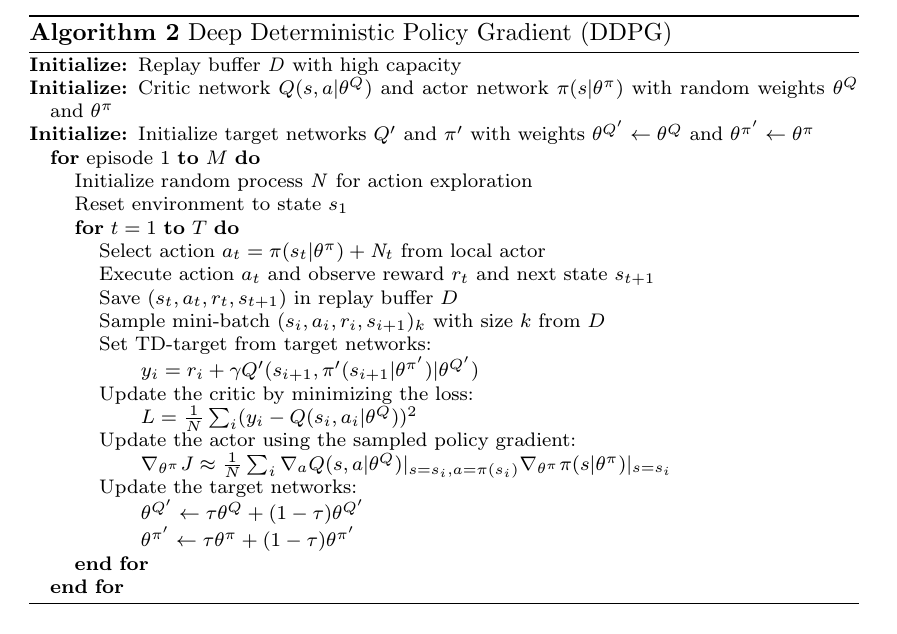
\includegraphics[scale=0.2]{ddpg_pseudocode.png}
	\end{frame}
	\begin{frame}
		\frametitle{\\Improvements for DDPG}
		\begin{itemize}
			\item \textbf{D4PG}
			\begin{itemize}
				\item Importance Weighted Experience Sampling
				\item Utilizing N-Step return
				\item Parallelized Actors
			\end{itemize}
		\end{itemize}
		\begin{multicols}{2}
			\begin{itemize}
				\item \textbf{Parameter Noise for Exploration}
				\\
				\hspace*{0.5 cm}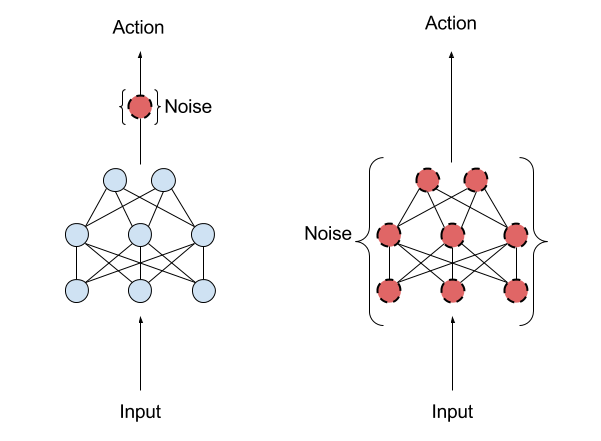
\includegraphics[scale=0.2]{parameter_noise.png}
				\item \textbf{Deep Changes}
				\\
				\vspace*{0.5cm}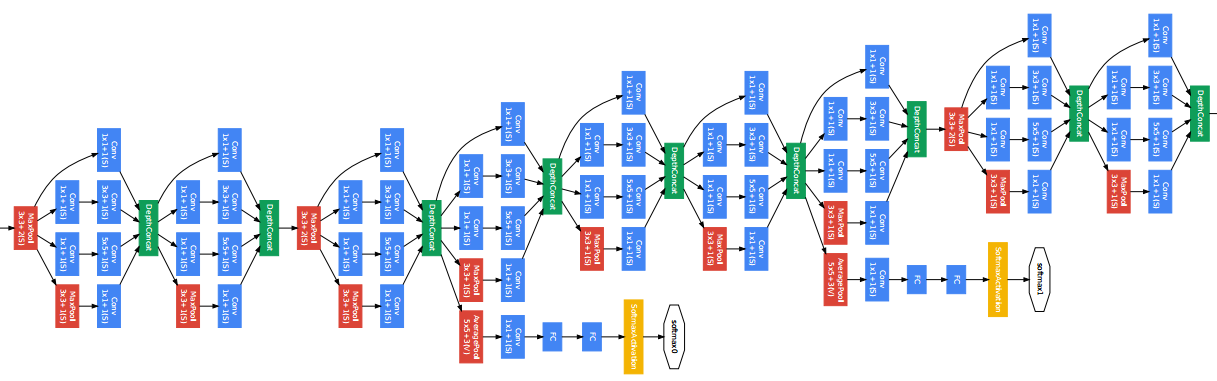
\includegraphics[scale=0.12]{googlenet.png} 
			\end{itemize}
		\end{multicols}
	\end{frame}
	\begin{frame}
		\frametitle{\\Sources}
		\begin{itemize}
			\item For publication references please see our paper "Deep Deterministic Policy Gradients: Components and Extensions"
			\item GoogLenet: https://towardsdatascience.com/an-intuitive-guide-to-deep-network-architectures-65fdc477db41
			\item Parameter noise for exploration:
			https://openai.com/blog/better-exploration-with-parameter-noise/			
		\end{itemize}

	\end{frame}
\end{document}